\documentclass[a4paper,12pt]{article}
\usepackage[utf8]{inputenc}

\usepackage[utf8]{inputenc}
\usepackage[T2A]{fontenc}
\usepackage[english,russian]{babel}
\usepackage{amsthm}
\usepackage{amsmath}
\usepackage{amssymb}
\usepackage{tikz}
\usepackage{textcomp}
\usepackage{marvosym}
\usepackage{ esint }
\usepackage{mathtext}
\usepackage{siunitx} % Required for alignment
\usepackage{subfigure}
\usepackage{multirow}
\usepackage{rotating}
\usepackage{afterpage}
\usepackage[arrowdel]{physics}
\usepackage{booktabs}
\setlength{\topmargin}{-0.5in}
\setlength{\textheight}{9.1in}
\setlength{\oddsidemargin}{-0.4in}
\setlength{\evensidemargin}{-0.4in}
\setlength{\textwidth}{7in}
\setlength{\parindent}{0ex}
\setlength{\parskip}{1ex}
\newcommand{\ndiv}{\hspace{-4pt}\not|\hspace{2pt}}
\usepackage{floatrow,graphicx,calc}
\usepackage{float}
\usepackage[export]{adjustbox}
\usepackage{wrapfig}
\usepackage{pgfplots}
\usepackage{caption}
\pgfplotsset{compat=1.16}
\graphicspath{ {./images/} }
\RequirePackage{caption}
\DeclareCaptionLabelSeparator{defffis}{ — }
\captionsetup{justification=centering,labelsep=defffis}
\usepackage{caption} \captionsetup[table]{labelsep=endash,justification=justified,singlelinecheck=false,font=normalsize}
\usepackage{amsfonts,mathtools}

\title{Лабораторная работа № 5.8.1\\ Тепловое излучение}
\author{Илья Прамский}
\date{Ноябрь 2024}

\begin{document}
\maketitle
\newpage
\section{Теоретическая справка}

По результатам измерений мощности излучения вольфрамовой нити можно судить о справедливости закона Стефана-Больцмана. Если бы нить излучала как АЧТ, то баланс потребляемой и излучаемой энергии определялся бы соотношением 
\begin{equation}
    W = \sigma S (T^4 - T_0^4),
\end{equation}
где $W$ - потребляемая нитью электрическая мощность, $S$ - площадь излучающей поверхности нити, $T$ - температура нити, $T_0$ - температура окружающей среды. Однако вольфрамовая нить излучает как серое тело, и излучение её ослаблено по сравнению с АЧТ в $\varepsilon_T$ раз для любой волны при данной температуре тела Т. Тогда предположив, что нить излучает как серое тело и с учётом того, что $T_0 \ll T$, выражение (1) можно переписать в виде
\begin{equation}
    W = \varepsilon_T S \sigma T^4
\end{equation}

\begin{figure}[H]
\centering
\includegraphics[scale=0.75]{scheme.png}
\end{figure}
\newpage
\section{Ход работы}
\subsection*{Проверка работы оптического пирометра}
Измерим температуру АЧТ при помощи оптического пирометра, а также с помощью термопары хромель-алюмель. Получилось (учитывая также добавку к значению термопары, равную комнатной температуре $T_k = 24^\circ C$)

\[T_\text{опт. пир.} = 1125^\circ C\]
\[T_\text{терм} = 1119^\circ C\]

\begin{figure}[H]
\centering
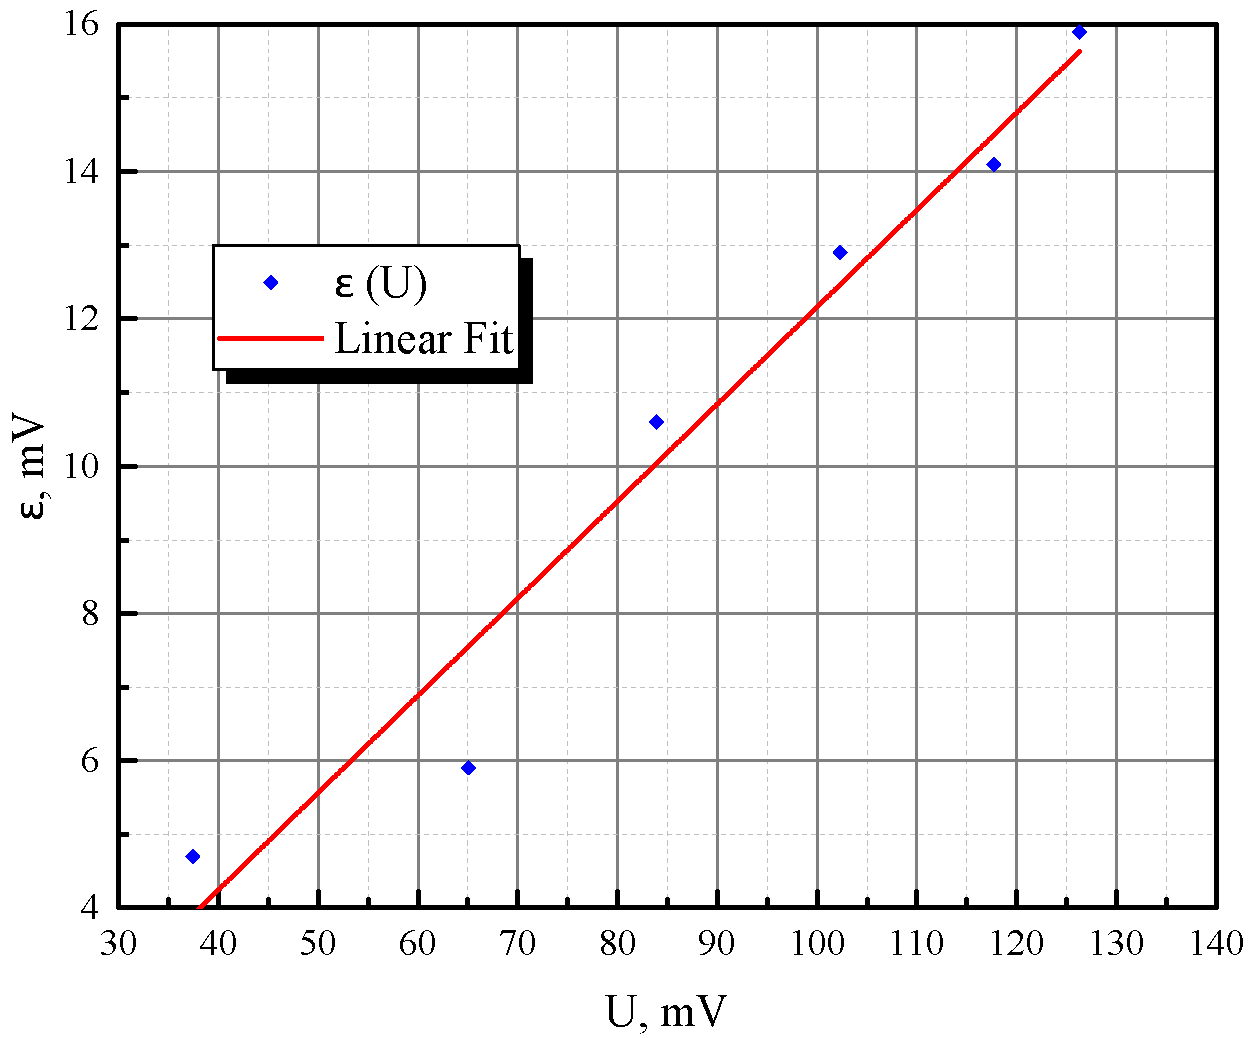
\includegraphics[scale=0.2]{graph.jpg}
\end{figure}

\subsection*{Измерение яркостной температуры накаленных тел}
Нагрев трубку и кольца до высокой температуры, получаем
\[T_\text{трубки} = 800^\circ C\]
\[T_\text{колец} < 800 ^\circ C\text{(не получилось определить при помощи пирометра)}\]
Разницу яркостных температур у различных тел, имеющих одинаковую термодинамическую температуру, вытекает из того, что данные материалы имеют разный спектральный коэффициент поглощения, который связывает эти 2 величины.

\subsection*{Проверка закона Стефана-Больцмана}
Построим график зависимости $\ln W = f(\ln T_\text{терм})$.

\begin{figure}[H]
    \centering
    \includegraphics[scale=0.5]{graphik.png}
    \caption{График зависимости $T=f(T_\text{ярк})$ для вольфрама}
\end{figure}

\begin{table}[H]
    \centering
    \begin{tabular}{|c|c|c|c|c|c|c|c|c|}
        \hline
        U, В & $\sigma_U$, В & I, мA & $\sigma_I$, мA & W, Вт & $\sigma_W$, Вт & $T_\text{ярк}$, К & $T_\text{терм}$, К & $\sigma_{T_\text{терм}}$, K \\
        \hline 
        1,66 & 0,04 & 472  & 3 & 0,78 & 0,02 & 1232 & 1270 & 5 \\
        \hline
        2,21 & 0,04 & 534  & 4 & 1,18 & 0,02 & 1366 & 1413 & 5 \\
        \hline
        2,53 & 0,04 & 569  & 4 & 1,44 & 0,03 & 1410 & 1460 & 5 \\
        \hline
        3,12 & 0,04 & 630  & 4 & 1,97 & 0,03 & 1519 & 1576 & 5 \\
        \hline
        3,68 & 0,04 & 683  & 4 & 2,51 & 0,03 & 1637 & 1702 & 5 \\
        \hline
        4,14 & 0,04 & 725  & 5 & 3,00 & 0,04 & 1720 & 1790 & 5 \\
        \hline
        4,54 & 0,04 & 760  & 5 & 3,45 & 0,04 & 1729 & 1800 & 5 \\
        \hline
        5,09 & 0,04 & 806  & 5 & 4,10 & 0,04 & 1853 & 1932 & 5 \\
        \hline
        6,02 & 0,04 & 880  & 5 & 5,30 & 0,05 & 1936 & 2021 & 5 \\
        \hline
        6,87 & 0,04 & 994  & 6 & 6,83 & 0,06 & 2008 & 2098 & 5 \\
        \hline
        7,70 & 0,04 & 1003 & 6 & 7,72 & 0,06 & 2083 & 2178 & 5 \\
        \hline
        8,70 & 0,04 & 1068 & 6 & 9,29 & 0,07 & 2153 & 2253 & 5 \\
        \hline
        8,78 & 0,04 & 1071 & 6 & 9,40 & 0,07 & 2209 & 2312 & 5 \\
        \hline
    \end{tabular}
\end{table}

\begin{figure}[H]
    \centering
    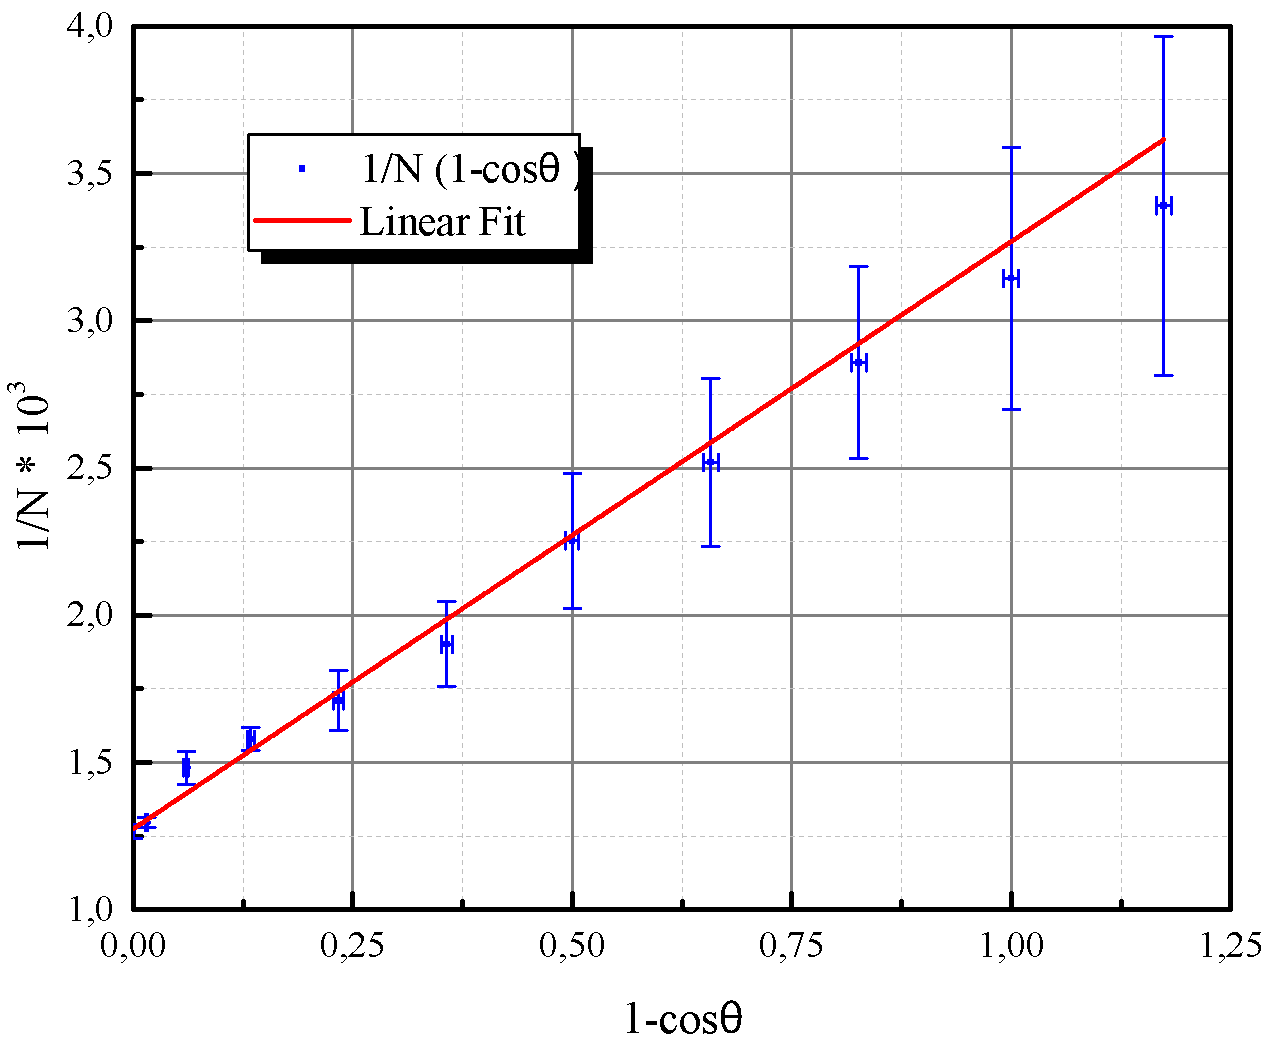
\includegraphics[scale=0.5]{graph1.png}
\end{figure}

Из графика: $n = 4,23 \pm 0,09$.
Найдём значение постоянной Стефана-Больцмана $\sigma$ для измерений при $T > 1700$ К. $S = 0,36 \text{см}^2$.

\begin{table}[H]
    \centering
    \begin{tabular}{|c|c|c|}
        \hline
        $T_\text{терм}$, K & $\sigma$, $10^{-12}$ $\frac{\text{Вт}}{\text{см}^2 \cdot K^4}$ & $\sigma_\sigma$, $10^{-12}$ $\frac{\text{Вт}}{\text{см}^2 \cdot K^4}$ \\
        \hline
        1702 & 3,98 & 0,05 \\
        \hline
        1790 & 3,67 & 0,06 \\
        \hline
        1800 & 4,09 & 0,07 \\
        \hline
        1932 & 3,46 & 0,05 \\
        \hline
        2021 & 3,5 & 0,05 \\
        \hline
    \end{tabular}
\end{table}
Получилось $\sigma = 3,74 \pm 0,03 \cdot 10^{-12}$ $\frac{\text{Вт}}{\text{см}^2 \cdot K^4}$.
Тогда $h = \sqrt[3]{\frac{2 \pi^5 k_\text{Б}^4}{15c^2 \sigma}} = 7,60 \pm 0,02 \cdot 10^{-34}$ Дж $\cdot$ с 
\subsection*{Измерения яркостной температуры неоновой лампочки}
Яркостная температура неоновой лампочки получилась равной $T_\text{ярк} = 973^\circ C$, когда термодинамическая температура равна комнатной(проверил пальцем). Это можно объяснить тем, что неоновая лампочка не является моделью чёрного или серого тела, её излучение носит другую природу(переход электронов между электронными уровнями).
\newpage
\section{Вывод}
В ходе работы было исследовано тепловое излучение, проверен закон Стефана-Больцмана(в итоге получилось соответствие данному закону, т.к. $n \approx 4$). Также был найден коэффициент Стефана-Больцмана $\sigma = 3,74 \pm 0,03 \cdot 10^{-12}$ $\frac{\text{Вт}}{\text{см}^2 \cdot K^4}$(Табличное же значение достаточно близко: $\sigma = 5,76 \cdot 10^{-12}$ $\frac{\text{Вт}}{\text{см}^2 \cdot K^4}$). 

В конце концов, была найдена постоянная Планка $h = 7,60 \pm 0,02 \cdot 10^{-34}$ Дж $\cdot$ с.


\end{document}